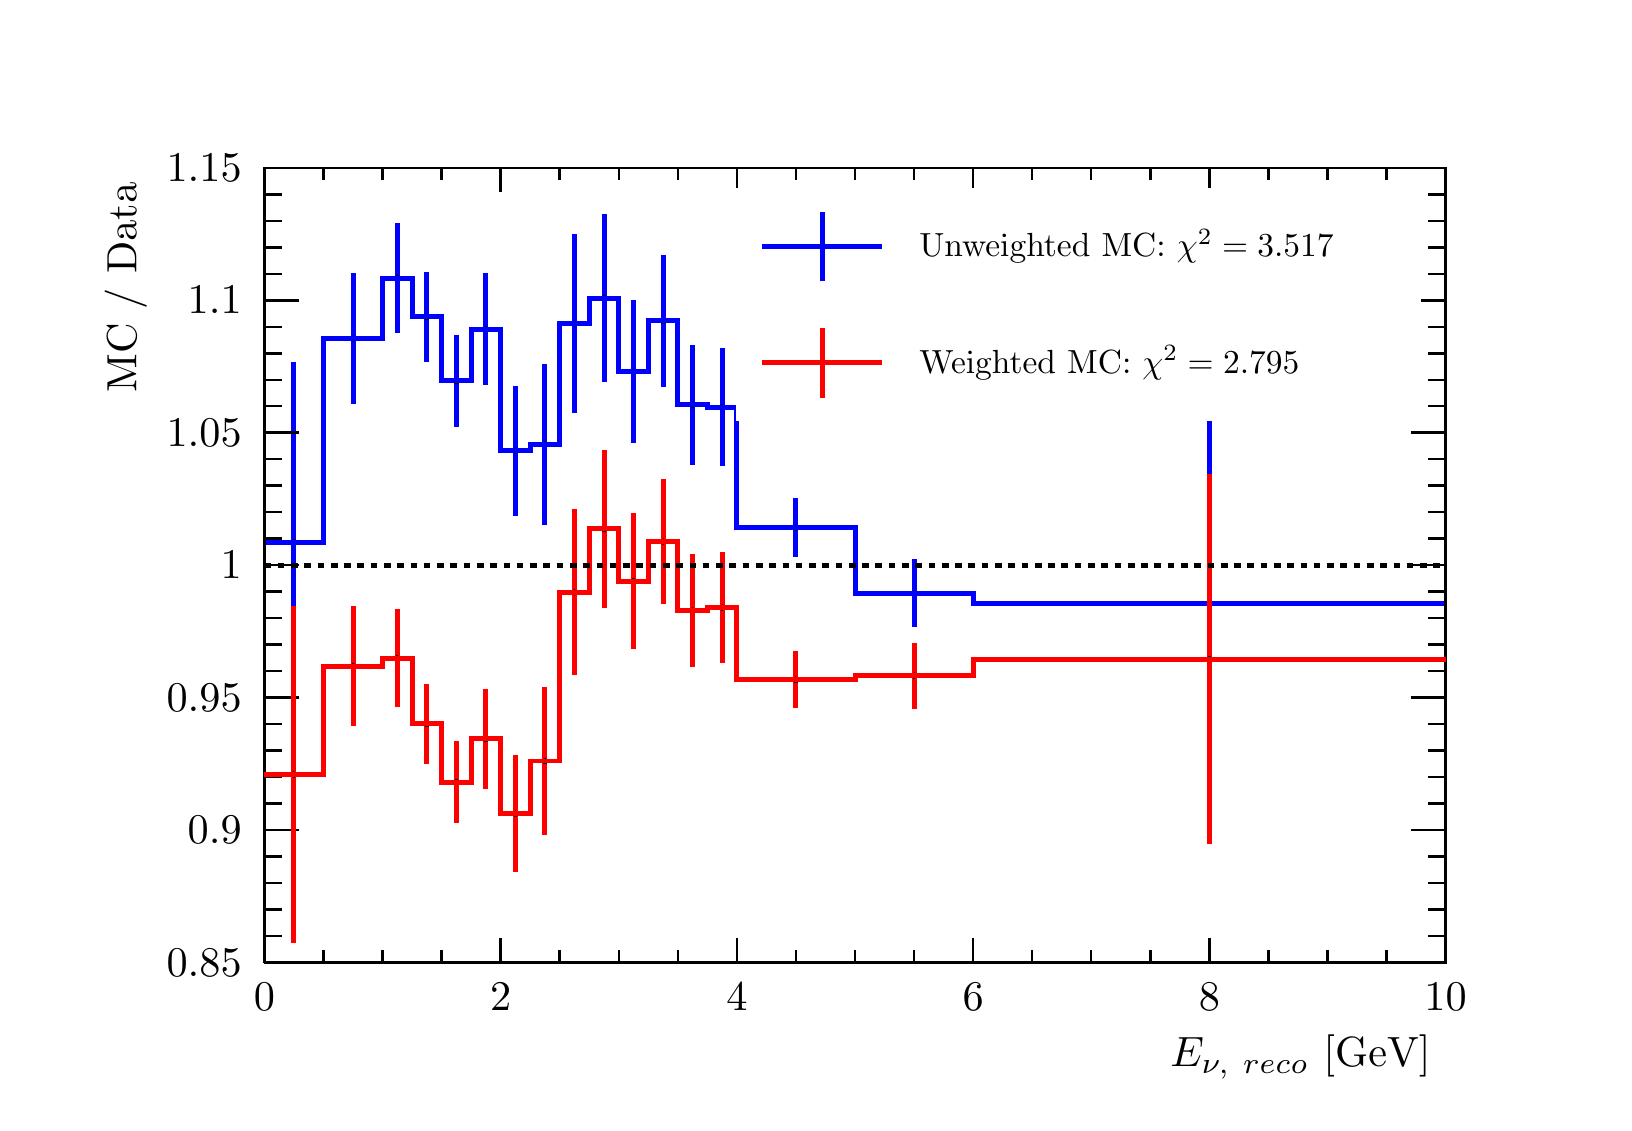
\begin{tikzpicture}
\pgfdeclareplotmark{cross} {
\pgfpathmoveto{\pgfpoint{-0.3\pgfplotmarksize}{\pgfplotmarksize}}
\pgfpathlineto{\pgfpoint{+0.3\pgfplotmarksize}{\pgfplotmarksize}}
\pgfpathlineto{\pgfpoint{+0.3\pgfplotmarksize}{0.3\pgfplotmarksize}}
\pgfpathlineto{\pgfpoint{+1\pgfplotmarksize}{0.3\pgfplotmarksize}}
\pgfpathlineto{\pgfpoint{+1\pgfplotmarksize}{-0.3\pgfplotmarksize}}
\pgfpathlineto{\pgfpoint{+0.3\pgfplotmarksize}{-0.3\pgfplotmarksize}}
\pgfpathlineto{\pgfpoint{+0.3\pgfplotmarksize}{-1.\pgfplotmarksize}}
\pgfpathlineto{\pgfpoint{-0.3\pgfplotmarksize}{-1.\pgfplotmarksize}}
\pgfpathlineto{\pgfpoint{-0.3\pgfplotmarksize}{-0.3\pgfplotmarksize}}
\pgfpathlineto{\pgfpoint{-1.\pgfplotmarksize}{-0.3\pgfplotmarksize}}
\pgfpathlineto{\pgfpoint{-1.\pgfplotmarksize}{0.3\pgfplotmarksize}}
\pgfpathlineto{\pgfpoint{-0.3\pgfplotmarksize}{0.3\pgfplotmarksize}}
\pgfpathclose
\pgfusepathqstroke
}
\pgfdeclareplotmark{cross*} {
\pgfpathmoveto{\pgfpoint{-0.3\pgfplotmarksize}{\pgfplotmarksize}}
\pgfpathlineto{\pgfpoint{+0.3\pgfplotmarksize}{\pgfplotmarksize}}
\pgfpathlineto{\pgfpoint{+0.3\pgfplotmarksize}{0.3\pgfplotmarksize}}
\pgfpathlineto{\pgfpoint{+1\pgfplotmarksize}{0.3\pgfplotmarksize}}
\pgfpathlineto{\pgfpoint{+1\pgfplotmarksize}{-0.3\pgfplotmarksize}}
\pgfpathlineto{\pgfpoint{+0.3\pgfplotmarksize}{-0.3\pgfplotmarksize}}
\pgfpathlineto{\pgfpoint{+0.3\pgfplotmarksize}{-1.\pgfplotmarksize}}
\pgfpathlineto{\pgfpoint{-0.3\pgfplotmarksize}{-1.\pgfplotmarksize}}
\pgfpathlineto{\pgfpoint{-0.3\pgfplotmarksize}{-0.3\pgfplotmarksize}}
\pgfpathlineto{\pgfpoint{-1.\pgfplotmarksize}{-0.3\pgfplotmarksize}}
\pgfpathlineto{\pgfpoint{-1.\pgfplotmarksize}{0.3\pgfplotmarksize}}
\pgfpathlineto{\pgfpoint{-0.3\pgfplotmarksize}{0.3\pgfplotmarksize}}
\pgfpathclose
\pgfusepathqfillstroke
}
\pgfdeclareplotmark{newstar} {
\pgfpathmoveto{\pgfqpoint{0pt}{\pgfplotmarksize}}
\pgfpathlineto{\pgfqpointpolar{44}{0.5\pgfplotmarksize}}
\pgfpathlineto{\pgfqpointpolar{18}{\pgfplotmarksize}}
\pgfpathlineto{\pgfqpointpolar{-20}{0.5\pgfplotmarksize}}
\pgfpathlineto{\pgfqpointpolar{-54}{\pgfplotmarksize}}
\pgfpathlineto{\pgfqpointpolar{-90}{0.5\pgfplotmarksize}}
\pgfpathlineto{\pgfqpointpolar{234}{\pgfplotmarksize}}
\pgfpathlineto{\pgfqpointpolar{198}{0.5\pgfplotmarksize}}
\pgfpathlineto{\pgfqpointpolar{162}{\pgfplotmarksize}}
\pgfpathlineto{\pgfqpointpolar{134}{0.5\pgfplotmarksize}}
\pgfpathclose
\pgfusepathqstroke
}
\pgfdeclareplotmark{newstar*} {
\pgfpathmoveto{\pgfqpoint{0pt}{\pgfplotmarksize}}
\pgfpathlineto{\pgfqpointpolar{44}{0.5\pgfplotmarksize}}
\pgfpathlineto{\pgfqpointpolar{18}{\pgfplotmarksize}}
\pgfpathlineto{\pgfqpointpolar{-20}{0.5\pgfplotmarksize}}
\pgfpathlineto{\pgfqpointpolar{-54}{\pgfplotmarksize}}
\pgfpathlineto{\pgfqpointpolar{-90}{0.5\pgfplotmarksize}}
\pgfpathlineto{\pgfqpointpolar{234}{\pgfplotmarksize}}
\pgfpathlineto{\pgfqpointpolar{198}{0.5\pgfplotmarksize}}
\pgfpathlineto{\pgfqpointpolar{162}{\pgfplotmarksize}}
\pgfpathlineto{\pgfqpointpolar{134}{0.5\pgfplotmarksize}}
\pgfpathclose
\pgfusepathqfillstroke
}
\definecolor{c}{rgb}{1,1,1};
\draw [color=c, fill=c] (0,0) rectangle (20,13.639);
\draw [color=c, fill=c] (3,1.77307) rectangle (18,11.8659);
\definecolor{c}{rgb}{0,0,0};
\draw [c,line width=0.9] (3,1.77307) -- (3,11.8659) -- (18,11.8659) -- (18,1.77307) -- (3,1.77307);
\definecolor{c}{rgb}{1,1,1};
\draw [color=c, fill=c] (3,1.77307) rectangle (18,11.8659);
\definecolor{c}{rgb}{0,0,0};
\draw [c,line width=0.9] (3,1.77307) -- (3,11.8659) -- (18,11.8659) -- (18,1.77307) -- (3,1.77307);
\definecolor{c}{rgb}{0,0,1};
\draw [c,line width=1.8] (3.375,4.82235) -- (3.375,7.11133);
\draw [c,line width=1.8] (3.375,7.11133) -- (3.375,9.4003);
\definecolor{c}{rgb}{0,0,0};
\foreach \P in {(3.375,7.11133)}{\draw[mark options={color=c,fill=c},mark size=2.402402pt, line width=0.000000pt, mark=*,mark size=1pt] plot coordinates {\P};}
\definecolor{c}{rgb}{0,0,1};
\draw [c,line width=1.8] (4.125,8.86415) -- (4.125,9.69792);
\draw [c,line width=1.8] (4.125,9.69792) -- (4.125,10.5317);
\definecolor{c}{rgb}{0,0,0};
\foreach \P in {(4.125,9.69792)}{\draw[mark options={color=c,fill=c},mark size=2.402402pt, line width=0.000000pt, mark=*,mark size=1pt] plot coordinates {\P};}
\definecolor{c}{rgb}{0,0,1};
\draw [c,line width=1.8] (4.6875,9.77105) -- (4.6875,10.4651);
\draw [c,line width=1.8] (4.6875,10.4651) -- (4.6875,11.1591);
\definecolor{c}{rgb}{0,0,0};
\foreach \P in {(4.6875,10.4651)}{\draw[mark options={color=c,fill=c},mark size=2.402402pt, line width=0.000000pt, mark=*,mark size=1pt] plot coordinates {\P};}
\definecolor{c}{rgb}{0,0,1};
\draw [c,line width=1.8] (5.0625,9.40033) -- (5.0625,9.97166);
\draw [c,line width=1.8] (5.0625,9.97166) -- (5.0625,10.543);
\definecolor{c}{rgb}{0,0,0};
\foreach \P in {(5.0625,9.97166)}{\draw[mark options={color=c,fill=c},mark size=2.402402pt, line width=0.000000pt, mark=*,mark size=1pt] plot coordinates {\P};}
\definecolor{c}{rgb}{0,0,1};
\draw [c,line width=1.8] (5.4375,8.57753) -- (5.4375,9.1589);
\draw [c,line width=1.8] (5.4375,9.1589) -- (5.4375,9.74027);
\definecolor{c}{rgb}{0,0,0};
\foreach \P in {(5.4375,9.1589)}{\draw[mark options={color=c,fill=c},mark size=2.402402pt, line width=0.000000pt, mark=*,mark size=1pt] plot coordinates {\P};}
\definecolor{c}{rgb}{0,0,1};
\draw [c,line width=1.8] (5.8125,9.11223) -- (5.8125,9.81875);
\draw [c,line width=1.8] (5.8125,9.81875) -- (5.8125,10.5253);
\definecolor{c}{rgb}{0,0,0};
\foreach \P in {(5.8125,9.81875)}{\draw[mark options={color=c,fill=c},mark size=2.402402pt, line width=0.000000pt, mark=*,mark size=1pt] plot coordinates {\P};}
\definecolor{c}{rgb}{0,0,1};
\draw [c,line width=1.8] (6.1875,7.4464) -- (6.1875,8.27347);
\draw [c,line width=1.8] (6.1875,8.27347) -- (6.1875,9.10054);
\definecolor{c}{rgb}{0,0,0};
\foreach \P in {(6.1875,8.27347)}{\draw[mark options={color=c,fill=c},mark size=2.402402pt, line width=0.000000pt, mark=*,mark size=1pt] plot coordinates {\P};}
\definecolor{c}{rgb}{0,0,1};
\draw [c,line width=1.8] (6.5625,7.3329) -- (6.5625,8.35608);
\draw [c,line width=1.8] (6.5625,8.35608) -- (6.5625,9.37926);
\definecolor{c}{rgb}{0,0,0};
\foreach \P in {(6.5625,8.35608)}{\draw[mark options={color=c,fill=c},mark size=2.402402pt, line width=0.000000pt, mark=*,mark size=1pt] plot coordinates {\P};}
\definecolor{c}{rgb}{0,0,1};
\draw [c,line width=1.8] (6.9375,8.75536) -- (6.9375,9.89207);
\draw [c,line width=1.8] (6.9375,9.89207) -- (6.9375,11.0288);
\definecolor{c}{rgb}{0,0,0};
\foreach \P in {(6.9375,9.89207)}{\draw[mark options={color=c,fill=c},mark size=2.402402pt, line width=0.000000pt, mark=*,mark size=1pt] plot coordinates {\P};}
\definecolor{c}{rgb}{0,0,1};
\draw [c,line width=1.8] (7.3125,9.14294) -- (7.3125,10.2107);
\draw [c,line width=1.8] (7.3125,10.2107) -- (7.3125,11.2785);
\definecolor{c}{rgb}{0,0,0};
\foreach \P in {(7.3125,10.2107)}{\draw[mark options={color=c,fill=c},mark size=2.402402pt, line width=0.000000pt, mark=*,mark size=1pt] plot coordinates {\P};}
\definecolor{c}{rgb}{0,0,1};
\draw [c,line width=1.8] (7.6875,8.37385) -- (7.6875,9.28303);
\draw [c,line width=1.8] (7.6875,9.28303) -- (7.6875,10.1922);
\definecolor{c}{rgb}{0,0,0};
\foreach \P in {(7.6875,9.28303)}{\draw[mark options={color=c,fill=c},mark size=2.402402pt, line width=0.000000pt, mark=*,mark size=1pt] plot coordinates {\P};}
\definecolor{c}{rgb}{0,0,1};
\draw [c,line width=1.8] (8.0625,9.08244) -- (8.0625,9.92258);
\draw [c,line width=1.8] (8.0625,9.92258) -- (8.0625,10.7627);
\definecolor{c}{rgb}{0,0,0};
\foreach \P in {(8.0625,9.92258)}{\draw[mark options={color=c,fill=c},mark size=2.402402pt, line width=0.000000pt, mark=*,mark size=1pt] plot coordinates {\P};}
\definecolor{c}{rgb}{0,0,1};
\draw [c,line width=1.8] (8.4375,8.09525) -- (8.4375,8.85714);
\draw [c,line width=1.8] (8.4375,8.85714) -- (8.4375,9.61902);
\definecolor{c}{rgb}{0,0,0};
\foreach \P in {(8.4375,8.85714)}{\draw[mark options={color=c,fill=c},mark size=2.402402pt, line width=0.000000pt, mark=*,mark size=1pt] plot coordinates {\P};}
\definecolor{c}{rgb}{0,0,1};
\draw [c,line width=1.8] (8.8125,8.07856) -- (8.8125,8.82826);
\draw [c,line width=1.8] (8.8125,8.82826) -- (8.8125,9.57796);
\definecolor{c}{rgb}{0,0,0};
\foreach \P in {(8.8125,8.82826)}{\draw[mark options={color=c,fill=c},mark size=2.402402pt, line width=0.000000pt, mark=*,mark size=1pt] plot coordinates {\P};}
\definecolor{c}{rgb}{0,0,1};
\draw [c,line width=1.8] (9.75,6.92167) -- (9.75,7.29785);
\draw [c,line width=1.8] (9.75,7.29785) -- (9.75,7.67403);
\definecolor{c}{rgb}{0,0,0};
\foreach \P in {(9.75,7.29785)}{\draw[mark options={color=c,fill=c},mark size=2.402402pt, line width=0.000000pt, mark=*,mark size=1pt] plot coordinates {\P};}
\definecolor{c}{rgb}{0,0,1};
\draw [c,line width=1.8] (11.25,6.03502) -- (11.25,6.46348);
\draw [c,line width=1.8] (11.25,6.46348) -- (11.25,6.89195);
\definecolor{c}{rgb}{0,0,0};
\foreach \P in {(11.25,6.46348)}{\draw[mark options={color=c,fill=c},mark size=2.402402pt, line width=0.000000pt, mark=*,mark size=1pt] plot coordinates {\P};}
\definecolor{c}{rgb}{0,0,1};
\draw [c,line width=1.8] (15,3.94313) -- (15,6.32831);
\draw [c,line width=1.8] (15,6.32831) -- (15,8.71348);
\definecolor{c}{rgb}{0,0,0};
\foreach \P in {(15,6.32831)}{\draw[mark options={color=c,fill=c},mark size=2.402402pt, line width=0.000000pt, mark=*,mark size=1pt] plot coordinates {\P};}
\definecolor{c}{rgb}{0,0,1};
\draw [c,line width=1.8] (3,7.11133) -- (3.75,7.11133) -- (3.75,9.69792) -- (4.5,9.69792) -- (4.5,10.4651) -- (4.875,10.4651) -- (4.875,9.97166) -- (5.25,9.97166) -- (5.25,9.1589) -- (5.625,9.1589) -- (5.625,9.81875) -- (6,9.81875) -- (6,8.27347) --
 (6.375,8.27347) -- (6.375,8.35608) -- (6.75,8.35608) -- (6.75,9.89207) -- (7.125,9.89207) -- (7.125,10.2107) -- (7.5,10.2107) -- (7.5,9.28303) -- (7.875,9.28303) -- (7.875,9.92258) -- (8.25,9.92258) -- (8.25,8.85714) -- (8.625,8.85714) --
 (8.625,8.82826) -- (9,8.82826) -- (9,7.29785) -- (10.5,7.29785) -- (10.5,6.46348) -- (12,6.46348) -- (12,6.32831) -- (18,6.32831);
\definecolor{c}{rgb}{0,0,0};
\draw [c,line width=0.9] (3,1.77307) -- (18,1.77307);
\draw [c,line width=0.9] (3,2.07994) -- (3,1.77307);
\draw [c,line width=0.9] (3.75,1.9265) -- (3.75,1.77307);
\draw [c,line width=0.9] (4.5,1.9265) -- (4.5,1.77307);
\draw [c,line width=0.9] (5.25,1.9265) -- (5.25,1.77307);
\draw [c,line width=0.9] (6,2.07994) -- (6,1.77307);
\draw [c,line width=0.9] (6.75,1.9265) -- (6.75,1.77307);
\draw [c,line width=0.9] (7.5,1.9265) -- (7.5,1.77307);
\draw [c,line width=0.9] (8.25,1.9265) -- (8.25,1.77307);
\draw [c,line width=0.9] (9,2.07994) -- (9,1.77307);
\draw [c,line width=0.9] (9.75,1.9265) -- (9.75,1.77307);
\draw [c,line width=0.9] (10.5,1.9265) -- (10.5,1.77307);
\draw [c,line width=0.9] (11.25,1.9265) -- (11.25,1.77307);
\draw [c,line width=0.9] (12,2.07994) -- (12,1.77307);
\draw [c,line width=0.9] (12.75,1.9265) -- (12.75,1.77307);
\draw [c,line width=0.9] (13.5,1.9265) -- (13.5,1.77307);
\draw [c,line width=0.9] (14.25,1.9265) -- (14.25,1.77307);
\draw [c,line width=0.9] (15,2.07994) -- (15,1.77307);
\draw [c,line width=0.9] (15.75,1.9265) -- (15.75,1.77307);
\draw [c,line width=0.9] (16.5,1.9265) -- (16.5,1.77307);
\draw [c,line width=0.9] (17.25,1.9265) -- (17.25,1.77307);
\draw [c,line width=0.9] (18,2.07994) -- (18,1.77307);
\draw [anchor=base] (3,1.15931) node[scale=1.52731, color=c, rotate=0]{0};
\draw [anchor=base] (6,1.15931) node[scale=1.52731, color=c, rotate=0]{2};
\draw [anchor=base] (9,1.15931) node[scale=1.52731, color=c, rotate=0]{4};
\draw [anchor=base] (12,1.15931) node[scale=1.52731, color=c, rotate=0]{6};
\draw [anchor=base] (15,1.15931) node[scale=1.52731, color=c, rotate=0]{8};
\draw [anchor=base] (18,1.15931) node[scale=1.52731, color=c, rotate=0]{10};
\draw [anchor= east] (18,0.572837) node[scale=1.52731, color=c, rotate=0]{$E_{\nu,~\text{reco}}$ [GeV]};
\draw [c,line width=0.9] (3,11.8659) -- (18,11.8659);
\draw [c,line width=0.9] (3,11.559) -- (3,11.8659);
\draw [c,line width=0.9] (3.75,11.7125) -- (3.75,11.8659);
\draw [c,line width=0.9] (4.5,11.7125) -- (4.5,11.8659);
\draw [c,line width=0.9] (5.25,11.7125) -- (5.25,11.8659);
\draw [c,line width=0.9] (6,11.559) -- (6,11.8659);
\draw [c,line width=0.9] (6.75,11.7125) -- (6.75,11.8659);
\draw [c,line width=0.9] (7.5,11.7125) -- (7.5,11.8659);
\draw [c,line width=0.9] (8.25,11.7125) -- (8.25,11.8659);
\draw [c,line width=0.9] (9,11.559) -- (9,11.8659);
\draw [c,line width=0.9] (9.75,11.7125) -- (9.75,11.8659);
\draw [c,line width=0.9] (10.5,11.7125) -- (10.5,11.8659);
\draw [c,line width=0.9] (11.25,11.7125) -- (11.25,11.8659);
\draw [c,line width=0.9] (12,11.559) -- (12,11.8659);
\draw [c,line width=0.9] (12.75,11.7125) -- (12.75,11.8659);
\draw [c,line width=0.9] (13.5,11.7125) -- (13.5,11.8659);
\draw [c,line width=0.9] (14.25,11.7125) -- (14.25,11.8659);
\draw [c,line width=0.9] (15,11.559) -- (15,11.8659);
\draw [c,line width=0.9] (15.75,11.7125) -- (15.75,11.8659);
\draw [c,line width=0.9] (16.5,11.7125) -- (16.5,11.8659);
\draw [c,line width=0.9] (17.25,11.7125) -- (17.25,11.8659);
\draw [c,line width=0.9] (18,11.559) -- (18,11.8659);
\draw [c,line width=0.9] (3,1.77307) -- (3,11.8659);
\draw [c,line width=0.9] (3.444,1.77307) -- (3,1.77307);
\draw [c,line width=0.9] (3.222,2.10949) -- (3,2.10949);
\draw [c,line width=0.9] (3.222,2.44592) -- (3,2.44592);
\draw [c,line width=0.9] (3.222,2.78235) -- (3,2.78235);
\draw [c,line width=0.9] (3.222,3.11878) -- (3,3.11878);
\draw [c,line width=0.9] (3.444,3.45521) -- (3,3.45521);
\draw [c,line width=0.9] (3.222,3.79163) -- (3,3.79163);
\draw [c,line width=0.9] (3.222,4.12806) -- (3,4.12806);
\draw [c,line width=0.9] (3.222,4.46449) -- (3,4.46449);
\draw [c,line width=0.9] (3.222,4.80092) -- (3,4.80092);
\draw [c,line width=0.9] (3.444,5.13734) -- (3,5.13734);
\draw [c,line width=0.9] (3.222,5.47377) -- (3,5.47377);
\draw [c,line width=0.9] (3.222,5.8102) -- (3,5.8102);
\draw [c,line width=0.9] (3.222,6.14663) -- (3,6.14663);
\draw [c,line width=0.9] (3.222,6.48306) -- (3,6.48306);
\draw [c,line width=0.9] (3.444,6.81948) -- (3,6.81948);
\draw [c,line width=0.9] (3.222,7.15591) -- (3,7.15591);
\draw [c,line width=0.9] (3.222,7.49234) -- (3,7.49234);
\draw [c,line width=0.9] (3.222,7.82877) -- (3,7.82877);
\draw [c,line width=0.9] (3.222,8.1652) -- (3,8.1652);
\draw [c,line width=0.9] (3.444,8.50162) -- (3,8.50162);
\draw [c,line width=0.9] (3.222,8.83805) -- (3,8.83805);
\draw [c,line width=0.9] (3.222,9.17448) -- (3,9.17448);
\draw [c,line width=0.9] (3.222,9.51091) -- (3,9.51091);
\draw [c,line width=0.9] (3.222,9.84733) -- (3,9.84733);
\draw [c,line width=0.9] (3.444,10.1838) -- (3,10.1838);
\draw [c,line width=0.9] (3.222,10.5202) -- (3,10.5202);
\draw [c,line width=0.9] (3.222,10.8566) -- (3,10.8566);
\draw [c,line width=0.9] (3.222,11.193) -- (3,11.193);
\draw [c,line width=0.9] (3.222,11.5295) -- (3,11.5295);
\draw [c,line width=0.9] (3.444,11.8659) -- (3,11.8659);
\draw [c,line width=0.9] (3.444,1.77307) -- (3,1.77307);
\draw [c,line width=0.9] (3.444,11.8659) -- (3,11.8659);
\draw [anchor= east] (2.9,1.77307) node[scale=1.52731, color=c, rotate=0]{0.85};
\draw [anchor= east] (2.9,3.45521) node[scale=1.52731, color=c, rotate=0]{0.9};
\draw [anchor= east] (2.9,5.13734) node[scale=1.52731, color=c, rotate=0]{0.95};
\draw [anchor= east] (2.9,6.81948) node[scale=1.52731, color=c, rotate=0]{1};
\draw [anchor= east] (2.9,8.50162) node[scale=1.52731, color=c, rotate=0]{1.05};
\draw [anchor= east] (2.9,10.1838) node[scale=1.52731, color=c, rotate=0]{1.1};
\draw [anchor= east] (2.9,11.8659) node[scale=1.52731, color=c, rotate=0]{1.15};
\draw [anchor= east] (1.24,11.8659) node[scale=1.52731, color=c, rotate=90]{MC / Data};
\draw [c,line width=0.9] (18,1.77307) -- (18,11.8659);
\draw [c,line width=0.9] (17.556,1.77307) -- (18,1.77307);
\draw [c,line width=0.9] (17.778,2.10949) -- (18,2.10949);
\draw [c,line width=0.9] (17.778,2.44592) -- (18,2.44592);
\draw [c,line width=0.9] (17.778,2.78235) -- (18,2.78235);
\draw [c,line width=0.9] (17.778,3.11878) -- (18,3.11878);
\draw [c,line width=0.9] (17.556,3.45521) -- (18,3.45521);
\draw [c,line width=0.9] (17.778,3.79163) -- (18,3.79163);
\draw [c,line width=0.9] (17.778,4.12806) -- (18,4.12806);
\draw [c,line width=0.9] (17.778,4.46449) -- (18,4.46449);
\draw [c,line width=0.9] (17.778,4.80092) -- (18,4.80092);
\draw [c,line width=0.9] (17.556,5.13734) -- (18,5.13734);
\draw [c,line width=0.9] (17.778,5.47377) -- (18,5.47377);
\draw [c,line width=0.9] (17.778,5.8102) -- (18,5.8102);
\draw [c,line width=0.9] (17.778,6.14663) -- (18,6.14663);
\draw [c,line width=0.9] (17.778,6.48306) -- (18,6.48306);
\draw [c,line width=0.9] (17.556,6.81948) -- (18,6.81948);
\draw [c,line width=0.9] (17.778,7.15591) -- (18,7.15591);
\draw [c,line width=0.9] (17.778,7.49234) -- (18,7.49234);
\draw [c,line width=0.9] (17.778,7.82877) -- (18,7.82877);
\draw [c,line width=0.9] (17.778,8.1652) -- (18,8.1652);
\draw [c,line width=0.9] (17.556,8.50162) -- (18,8.50162);
\draw [c,line width=0.9] (17.778,8.83805) -- (18,8.83805);
\draw [c,line width=0.9] (17.778,9.17448) -- (18,9.17448);
\draw [c,line width=0.9] (17.778,9.51091) -- (18,9.51091);
\draw [c,line width=0.9] (17.778,9.84733) -- (18,9.84733);
\draw [c,line width=0.9] (17.556,10.1838) -- (18,10.1838);
\draw [c,line width=0.9] (17.778,10.5202) -- (18,10.5202);
\draw [c,line width=0.9] (17.778,10.8566) -- (18,10.8566);
\draw [c,line width=0.9] (17.778,11.193) -- (18,11.193);
\draw [c,line width=0.9] (17.778,11.5295) -- (18,11.5295);
\draw [c,line width=0.9] (17.556,11.8659) -- (18,11.8659);
\draw [c,line width=0.9] (17.556,1.77307) -- (18,1.77307);
\draw [c,line width=0.9] (17.556,11.8659) -- (18,11.8659);
\definecolor{c}{rgb}{1,0,0};
\draw [c,line width=1.8] (3.375,2.02414) -- (3.375,4.16319);
\draw [c,line width=1.8] (3.375,4.16319) -- (3.375,6.30223);
\definecolor{c}{rgb}{0,0,0};
\foreach \P in {(3.375,4.16319)}{\draw[mark options={color=c,fill=c},mark size=2.402402pt, line width=0.000000pt, mark=*,mark size=1pt] plot coordinates {\P};}
\definecolor{c}{rgb}{1,0,0};
\draw [c,line width=1.8] (4.125,4.77754) -- (4.125,5.53879);
\draw [c,line width=1.8] (4.125,5.53879) -- (4.125,6.30003);
\definecolor{c}{rgb}{0,0,0};
\foreach \P in {(4.125,5.53879)}{\draw[mark options={color=c,fill=c},mark size=2.402402pt, line width=0.000000pt, mark=*,mark size=1pt] plot coordinates {\P};}
\definecolor{c}{rgb}{1,0,0};
\draw [c,line width=1.8] (4.6875,5.01302) -- (4.6875,5.63814);
\draw [c,line width=1.8] (4.6875,5.63814) -- (4.6875,6.26325);
\definecolor{c}{rgb}{0,0,0};
\foreach \P in {(4.6875,5.63814)}{\draw[mark options={color=c,fill=c},mark size=2.402402pt, line width=0.000000pt, mark=*,mark size=1pt] plot coordinates {\P};}
\definecolor{c}{rgb}{1,0,0};
\draw [c,line width=1.8] (5.0625,4.29534) -- (5.0625,4.80524);
\draw [c,line width=1.8] (5.0625,4.80524) -- (5.0625,5.31514);
\definecolor{c}{rgb}{0,0,0};
\foreach \P in {(5.0625,4.80524)}{\draw[mark options={color=c,fill=c},mark size=2.402402pt, line width=0.000000pt, mark=*,mark size=1pt] plot coordinates {\P};}
\definecolor{c}{rgb}{1,0,0};
\draw [c,line width=1.8] (5.4375,3.54665) -- (5.4375,4.06522);
\draw [c,line width=1.8] (5.4375,4.06522) -- (5.4375,4.5838);
\definecolor{c}{rgb}{0,0,0};
\foreach \P in {(5.4375,4.06522)}{\draw[mark options={color=c,fill=c},mark size=2.402402pt, line width=0.000000pt, mark=*,mark size=1pt] plot coordinates {\P};}
\definecolor{c}{rgb}{1,0,0};
\draw [c,line width=1.8] (5.8125,3.98266) -- (5.8125,4.61236);
\draw [c,line width=1.8] (5.8125,4.61236) -- (5.8125,5.24206);
\definecolor{c}{rgb}{0,0,0};
\foreach \P in {(5.8125,4.61236)}{\draw[mark options={color=c,fill=c},mark size=2.402402pt, line width=0.000000pt, mark=*,mark size=1pt] plot coordinates {\P};}
\definecolor{c}{rgb}{1,0,0};
\draw [c,line width=1.8] (6.1875,2.92038) -- (6.1875,3.66495);
\draw [c,line width=1.8] (6.1875,3.66495) -- (6.1875,4.40952);
\definecolor{c}{rgb}{0,0,0};
\foreach \P in {(6.1875,3.66495)}{\draw[mark options={color=c,fill=c},mark size=2.402402pt, line width=0.000000pt, mark=*,mark size=1pt] plot coordinates {\P};}
\definecolor{c}{rgb}{1,0,0};
\draw [c,line width=1.8] (6.5625,3.3984) -- (6.5625,4.33273);
\draw [c,line width=1.8] (6.5625,4.33273) -- (6.5625,5.26705);
\definecolor{c}{rgb}{0,0,0};
\foreach \P in {(6.5625,4.33273)}{\draw[mark options={color=c,fill=c},mark size=2.402402pt, line width=0.000000pt, mark=*,mark size=1pt] plot coordinates {\P};}
\definecolor{c}{rgb}{1,0,0};
\draw [c,line width=1.8] (6.9375,5.41987) -- (6.9375,6.4758);
\draw [c,line width=1.8] (6.9375,6.4758) -- (6.9375,7.53172);
\definecolor{c}{rgb}{0,0,0};
\foreach \P in {(6.9375,6.4758)}{\draw[mark options={color=c,fill=c},mark size=2.402402pt, line width=0.000000pt, mark=*,mark size=1pt] plot coordinates {\P};}
\definecolor{c}{rgb}{1,0,0};
\draw [c,line width=1.8] (7.3125,6.27631) -- (7.3125,7.27948);
\draw [c,line width=1.8] (7.3125,7.27948) -- (7.3125,8.28265);
\definecolor{c}{rgb}{0,0,0};
\foreach \P in {(7.3125,7.27948)}{\draw[mark options={color=c,fill=c},mark size=2.402402pt, line width=0.000000pt, mark=*,mark size=1pt] plot coordinates {\P};}
\definecolor{c}{rgb}{1,0,0};
\draw [c,line width=1.8] (7.6875,5.75989) -- (7.6875,6.618);
\draw [c,line width=1.8] (7.6875,6.618) -- (7.6875,7.47611);
\definecolor{c}{rgb}{0,0,0};
\foreach \P in {(7.6875,6.618)}{\draw[mark options={color=c,fill=c},mark size=2.402402pt, line width=0.000000pt, mark=*,mark size=1pt] plot coordinates {\P};}
\definecolor{c}{rgb}{1,0,0};
\draw [c,line width=1.8] (8.0625,6.32838) -- (8.0625,7.1196);
\draw [c,line width=1.8] (8.0625,7.1196) -- (8.0625,7.91083);
\definecolor{c}{rgb}{0,0,0};
\foreach \P in {(8.0625,7.1196)}{\draw[mark options={color=c,fill=c},mark size=2.402402pt, line width=0.000000pt, mark=*,mark size=1pt] plot coordinates {\P};}
\definecolor{c}{rgb}{1,0,0};
\draw [c,line width=1.8] (8.4375,5.52791) -- (8.4375,6.24746);
\draw [c,line width=1.8] (8.4375,6.24746) -- (8.4375,6.96702);
\definecolor{c}{rgb}{0,0,0};
\foreach \P in {(8.4375,6.24746)}{\draw[mark options={color=c,fill=c},mark size=2.402402pt, line width=0.000000pt, mark=*,mark size=1pt] plot coordinates {\P};}
\definecolor{c}{rgb}{1,0,0};
\draw [c,line width=1.8] (8.8125,5.57304) -- (8.8125,6.28207);
\draw [c,line width=1.8] (8.8125,6.28207) -- (8.8125,6.99111);
\definecolor{c}{rgb}{0,0,0};
\foreach \P in {(8.8125,6.28207)}{\draw[mark options={color=c,fill=c},mark size=2.402402pt, line width=0.000000pt, mark=*,mark size=1pt] plot coordinates {\P};}
\definecolor{c}{rgb}{1,0,0};
\draw [c,line width=1.8] (9.75,5.00497) -- (9.75,5.36509);
\draw [c,line width=1.8] (9.75,5.36509) -- (9.75,5.72521);
\definecolor{c}{rgb}{0,0,0};
\foreach \P in {(9.75,5.36509)}{\draw[mark options={color=c,fill=c},mark size=2.402402pt, line width=0.000000pt, mark=*,mark size=1pt] plot coordinates {\P};}
\definecolor{c}{rgb}{1,0,0};
\draw [c,line width=1.8] (11.25,4.99932) -- (11.25,5.41769);
\draw [c,line width=1.8] (11.25,5.41769) -- (11.25,5.83607);
\definecolor{c}{rgb}{0,0,0};
\foreach \P in {(11.25,5.41769)}{\draw[mark options={color=c,fill=c},mark size=2.402402pt, line width=0.000000pt, mark=*,mark size=1pt] plot coordinates {\P};}
\definecolor{c}{rgb}{1,0,0};
\draw [c,line width=1.8] (15,3.28037) -- (15,5.6278);
\draw [c,line width=1.8] (15,5.6278) -- (15,7.97523);
\definecolor{c}{rgb}{0,0,0};
\foreach \P in {(15,5.6278)}{\draw[mark options={color=c,fill=c},mark size=2.402402pt, line width=0.000000pt, mark=*,mark size=1pt] plot coordinates {\P};}
\definecolor{c}{rgb}{1,0,0};
\draw [c,line width=1.8] (3,4.16319) -- (3.75,4.16319) -- (3.75,5.53879) -- (4.5,5.53879) -- (4.5,5.63814) -- (4.875,5.63814) -- (4.875,4.80524) -- (5.25,4.80524) -- (5.25,4.06522) -- (5.625,4.06522) -- (5.625,4.61236) -- (6,4.61236) -- (6,3.66495)
 -- (6.375,3.66495) -- (6.375,4.33273) -- (6.75,4.33273) -- (6.75,6.4758) -- (7.125,6.4758) -- (7.125,7.27948) -- (7.5,7.27948) -- (7.5,6.618) -- (7.875,6.618) -- (7.875,7.1196) -- (8.25,7.1196) -- (8.25,6.24746) -- (8.625,6.24746) -- (8.625,6.28207)
 -- (9,6.28207) -- (9,5.36509) -- (10.5,5.36509) -- (10.5,5.41769) -- (12,5.41769) -- (12,5.6278) -- (18,5.6278);
\definecolor{c}{rgb}{0,0,0};
\draw [c,dash pattern=on 2.40pt off 2.40pt ,line width=1.8] (3,6.81948) -- (18,6.81948);
\definecolor{c}{rgb}{1,1,1};
\draw [color=c, fill=c] (8.99713,8.6533) rectangle (17.6791,11.6046);
\definecolor{c}{rgb}{0,0,0};
\draw [anchor= west] (11.1676,10.8668) node[scale=1.20912, color=c, rotate=0]{Unweighted MC: $\chi^{2} = 3.517$};
\definecolor{c}{rgb}{0,0,1};
\draw [c,line width=1.8] (9.32271,10.8668) -- (10.842,10.8668);
\draw [c,line width=1.8] (10.0824,10.4241) -- (10.0824,11.3095);
\definecolor{c}{rgb}{0,0,0};
\draw [anchor= west] (11.1676,9.39112) node[scale=1.20912, color=c, rotate=0]{Weighted MC: $\chi^{2} = 2.795$};
\definecolor{c}{rgb}{1,0,0};
\draw [c,line width=1.8] (9.32271,9.39112) -- (10.842,9.39112);
\draw [c,line width=1.8] (10.0824,8.94842) -- (10.0824,9.83381);
\definecolor{c}{rgb}{1,1,1};
\draw [color=c, fill=c] (2,12.8206) rectangle (18,13.5708);
\end{tikzpicture}
